%!TEX root = ../main.tex

\chapter{The background model before cuts}\label{chap:bkg:raw:ph2}

As already mentioned, a precise knowledge of background intensity and distribution is
essential to searches of faint signals. One main assumption of the \onbb-decay signal
analysis is the distribution of background events in the analysis window around \qbb\
being uniform, except for the known \Tl\ and \Bil\ \g\ lines. The primary role of the
background model is to verify this assumption by exploiting data outside this energy
region or filtered with a different event selection. The background model is also
complementary to assay measurements in determining the location of the most dangerous
background sources and learn how to improve experimental design and material selection in
similar future projects. Lastly, a good background model allows to isolate \nnbb-decay
events, estimate the half-life of the process and study their distribution as a source of
potential new-physics effects (see \cref{chap:theory}).
\newpar
A first background model has been built for the \phaseone\ data and published
in~\cite{Agostini2013a}. Later, a new and advanced model has been constructed to describe
the first 60~\kgyr\ of \phasetwo\ data before the LAr veto and PSD cuts, which has been
published in~\cite{Agostini2019b} and is described in detail in this chapter.

\section{Analysis data sets}%
\label{sec:bkg:raw:data}

\begin{table}[b]
  \centering
  \caption{%
    Properties of the data sets considered in this analysis. Further
    details about the \gerda\ detectors can be found in past
    publications~\cite{Agostini2013a, Agostini2018a}.
  }\label{tab:bkg:raw:ph2:datasets}
  \small
  \begin{tabular}{lccccc}
  \toprule
  \mr{2}{data set} & \mr{2}{composition}     & total Ge           & active \gesix\   & total Ge           & active \gesix\     \\
                   &                         & mass (kg)          & mass (kg)        & exposure (\kgyr)   & exposure (\kgyr)   \\
  \midrule
  \enrBEGeIIp\     & 29 \bege\footnotemark{} & $19.362 \pm 0.005$ & $17.17 \pm 0.32$ & $22.181 \pm 0.006$ & $17.31  \pm 0.32$  \\
  \enrSCoaxIIp\    & 6 \scoax\               & $11.827 \pm 0.002$ & $10.38 \pm 0.42$ & $13.179 \pm 0.003$ & $10.00  \pm 0.42$  \\
  \enrICoaxIIp\    & 4 \icoax\               & $ 7.802 \pm 0.002$ & $ 7.23 \pm 0.03$ & $ 8.775 \pm 0.002$ & $ 7.13  \pm 0.03$  \\
  \enrGeIIp\       & all enriched            & $38.991 \pm 0.006$ & $34.78 \pm 0.53$ & $44.135 \pm 0.007$ & $34.44  \pm 0.53$  \\
  \bottomrule
\end{tabular}

% vim: nowrap

\end{table}%
\footnotetext[1]{%
  The BEGe detector \GD{02D} is the only detector that does not fully
  deplete~\cite{Agostini2018a}. Hence, events triggered by this detector are
  not considered in either data set and it is omitted from the mass
  computation.
}

As already mentioned, the background model before cuts has been developed using data from
the first part of \phasetwo, namely, for data acquired starting from December 2015 to
March 2018. Single-detector (or multiplicity-one, abbreviated \Mone) events and
two-detector (multiplicity-two, abbreviated \Mtwo) events are considered for this
analysis. Events from the coaxial detectors with natural isotope composition, located in
the central detector string, are not used in this analysis due to large uncertainties on
their \nplus\ contact thickness and detection efficiency. The \Mone\ events are split in
two data sets based on the two enriched detector geometries which we call \enrBEGeII\ and
\enrCoaxII\ in the following.  The \Mtwo\ data form a third data set which is named
\enrGeII. The energy we associate to an \Mtwo\ event is the sum of the energies
reconstructed in the two detectors. The data sets, their exposure and respective detector
mass are listed in \cref{tab:bkg:raw:ph2:datasets}. Note that the \bege\ exposure of
31.1~\kgyr\ is higher than the one reported in~\cite{Agostini2019a} because additional
data for which PSD methods are not applicable is here included.

\begin{figure}
  \centering
  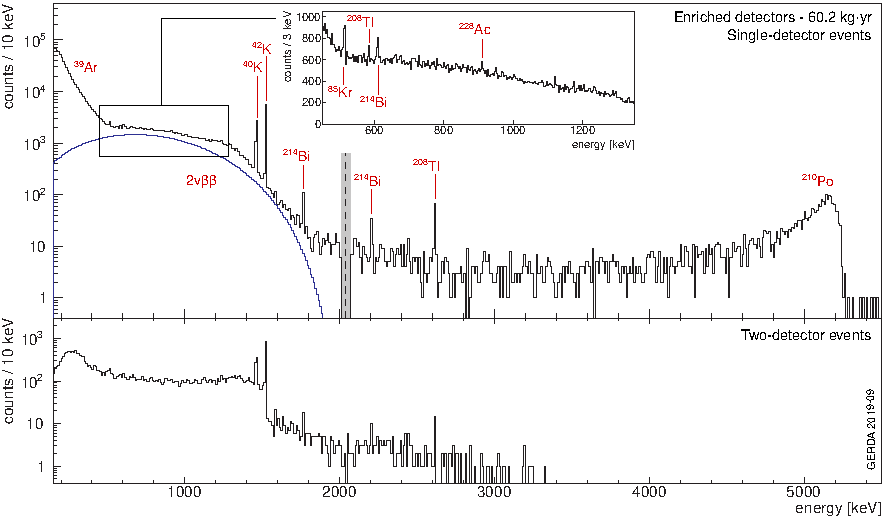
\includegraphics[width=0.9\linewidth]{plots/bkg/raw/ph2/dataGe-desc.pdf}
  \caption{%
    Summed energy spectra of single-detector events (\enrBEGeII\ and \enrCoaxII, top
    panel) and two-detector events (\enrGeII, bottom panel) collected in \gerda\
    \phasetwo.  The prominent features due to detector intrinsic \nnbb\ events, \kvz,
    \Arl\ and \Kr\ in the LAr, \kvn, the \Thh\ and \Uh\ decay chains are highlighted. The
    window blinded for the \onbb\ analysis is marked in grey.
  }\label{fig:bkg:raw:ph2:datasets}
\end{figure}

The event energy distribution of the three data sets is displayed in
\cref{fig:bkg:raw:ph2:datasets}; the sum spectrum of \enrBEGeII\ and \enrCoaxII\ in the
top panel and \enrGeII\ in the bottom panel. For the single-detector data, in the top
panel, the following features are most noticeable: the \b\ decay of \Arl\ dominates the
spectrum up to 565~keV while between 600 and 1500~keV the most prominent component is the
continuous spectrum of \nnbb\ decay of \gesix. Two \g\ lines at 1461 and 1525~keV can be
attributed to \kvn\ and \kvz; further visible \g\ lines belonging to \Kr, \Tl, \Bih\ and
\Ac\ are indicated in the figure. The highest energies displayed are dominated by a
peak-like structure emerging at 5.3~MeV with a pronounced low energy tail. This is a
typical spectral feature of \a\ particles and can, here, be attributed to \Po\ decay on
the thin detector \pplus\ surfaces~\cite{Agostini2013a}.  Events above the \Po\ peak
belong to \a\ decays emerging from the \Ra\ sub-chain on the detector \pplus\ surfaces.
All these components contribute also to \enrGeII\ except for \Arl, \nnbb\ and high energy
\a-components. This is due to the short range of \a\ (tens of \mum) and \b\
particles (typically smaller than 1.5~cm) in LAr and germanium with respect to the
distance between detectors which is of the order of several cm.

\section{Monte Carlo simulations and probability density functions}

The probability density functions (pdfs) used to model contributions to the energy spectra
are obtained from Monte Carlo simulations. The latter are performed using the \mage\
simulation framework~\cite{Boswell2011}, based on
\geant~\texttt{v10.4}~\cite{Agostinelli2002, Allison2006, Allison2016}.  \mage\ contains a
software implementation of the \gerdatwo\ detectors as well as the assembly and all other
surrounding hardware components. A visualization of this implementation is presented in
\cref{fig:setup:magevolumes}. Detector intrinsic \nnbb\ decays of \gesix\ and background
events originating from radioactive contaminations in and around the detector assembly are
simulated. The energy spectrum of the two electrons emitted in the \nnbb\ decay was
sampled according to the distribution given in~\cite{Tretyak1995} and implemented in
\decayzero~\cite{Ponkratenko2000}. The pdfs are obtained from the Monte Carlo simulations,
taking into account the finite energy resolution and individual exposure acquired with
each detector during the considered data taking periods. Special care is taken not to
statistically bias the pdfs by assuring that each simulated decay is taken into account
only once in the production of a pdf. For more details see \cref{apdx:magepdfs}.

\section{Background expectation}%
\label{sec:bkg:raw:ph2:priors}

The structural components of the setup have been screened for their radio-purity before
deployment. Two measurement methods were used depending on the screened isotope: \g-ray
spectroscopy (Ge-\g) with High Purity Germanium (in four underground laboratories, for
details see reference~\cite{Ackermann2012}) and mass spectrometry with Inductively Coupled
Plasma Mass Spectrometers (ICP-MS)~\cite{Vacri2015}. Especially materials close to the
detectors have been screened for radioactive contaminations originating from the \Uh\ and
\Thh\ decay chains, \kvn\ and \Co. For measured activities and upper limits see
reference~\cite{Agostini2018a} Sec.~5. All possible background sources taken into
consideration in this analysis are described in detail below. The descriptions are
accompanied by a selection of pdfs in \cref{fig:bkg:raw:ph2:pdfs:gmodel} (see also
\cref{apdx:magepdfs}).

\blocktitle{\Thh\ \\ \Uh}
The only isotopes simulated are \Pa, \Pbh\ and \Bih\ from the \Uh\ decay chain and \Ac,
\Bil\ and \Tl\ from the \Thh\ decay chain. The following groups of isotopes are assumed to
be in secular equilibrium: [\Uh, \Pa] [\Ra, \Pbh, \Bih] [$^{228}$Ra, \Ac] and [\Th, \Bil,
\Tl]. Their decay products consist of \g\  or \b\ particles with an energy higher than
520~keV. Less energetic particles from the remaining constituents in the chain do not
enter the energy window which is considered in the presented analysis. The \a\ emitters
from the decay chains contaminating the thin \pplus\ electrodes are described below.

\blocktitle{\Co}
A significant fraction of components in the \gerda\ setup is made of
copper~\cite{Agostini2018a}, which can be produced with high radio-purity but is
potentially activated by cosmic rays producing the long-lived isotope \Co. The latter
decays with a half-life of 5.2711(8)~yr; from material screening it is also expected to be
found in some of the detector high-voltage flexible flat cables.

\blocktitle{\kvn}
This isotope is found in all screened materials.  Construction materials were not
optimized for ultra-low \kvn\ content because the Q-value of its decay is well below \qbb\
and hence does not contribute to the background in the ROI. The \kvn\ decay spectrum
exhibits a \g\ line at 1460.822(6)~keV with an accumulated statistics on the order of
100~cts/detector. In \cref{fig:bkg:raw:ph2:pdfs:kmodel} the expected counts per detector
channel for \kvn\ simulated in different locations are shown. Using the ratio of events
detected in different detectors, information about the spatial distribution of \kvn\ can
be extracted. We use this spatial information to resolve degeneracies of \kvn\ in the
energy spectra (for details see \cref{apdx:kmodel}).

\blocktitle{\kvz}
A cosmogenically produced isotope in LAr is \Arh\ ($T_{1/2} = 32.9(11)$~yr) which decays
to \kvz. The distribution of \kvz\ inside the LAr is likely to be inhomogeneous due to
drift of the ionized decay products induced by the electric field (generated by
high-voltage cables and detectors) and convection. \kvz\ decays to $^{42}$Ca via \b\ decay
with a half-life of 12.355(7)~h and a Q-value of 3525.22(18)~keV, well above \qbb. For the
\b\ particle to be detected the decay needs to happen within a distance of a few
centimeters\footnote{The path length of \kvz\ \b\ particles in LAr is less than 1.6~cm,
but bremsstrahlung photons from the interaction with LAr can travel as far as
$\sim$10~cm.} to the detector surface. As the detectors are in direct contact with the
LAr, the \b\ component of \kvz\ potentially gives one of the most significant
contributions to the background in the ROI. Therefore, we separate decays originating
inside and outside the mini-shrouds in the following analysis. The full-range fit has
little sensitivity to any potassium inhomogeneity outside the mini-shrouds. \kvz\ is hence
assumed to be distributed homogeneously in this region. Based on detector-wise
observations, however, a surplus of \kvz\ above the detector array in the vicinity of the
front-end electronics is deduced (see \cref{apdx:kmodel}). Inside the mini-shrouds the \b\
spectrum becomes potentially important.  Some scenarios are possible, the closer \kvz\
decays to the detector surface, namely to the \nplus\ and \pplus\ contacts, the more \b\
particles enter the germanium. A fraction of events around \qbb\ coming from \kvz\ is
potentially due to \g\ particles with higher energy and sub-percent level branching ratio
or simultaneous energy deposition of multiple \g\ particles. This \g\ component could
become important for large quantities of \kvz\ not located directly on the detector
surfaces with the \b\ particle being absorbed in the LAr. As for \kvn\ also the \g\ line
at 1525~keV of \kvz\ contains valuable information about the spatial decay distribution of
this isotope. In contrast to \kvn\ no additional information, e.g.~from radio-purity
screening measurements, is available. For more detailed information about \kvn\ and \kvz\
see \cref{apdx:kmodel}.

\blocktitle{\a\ emitters}
The lithium-diffused \nplus\ detector surfaces act as a barrier for \a\ particles. The
latter can only penetrate the very thin boron-implanted \pplus-contact or the contact
separating groove. \a\ particles have to be emitted directly at the surface or from a thin
adjacent layer of LAr. Since \a\ particles have to cross the $\sim 0.5$~\mum\ thick
\pplus\ dead layer and therefore only part of their initial energy is deposited in the
active volume, this background component leads to peaks with characteristic low-energy
tails in the HPGe energy spectra (see \cref{fig:bkg:raw:ph2:pdfs:amodel:Po}). Some \a\
events, presumably originating from the detector groove, are reconstructed with degraded
energy and lead to an additional, continuous spectral component. We find mainly \Po\ but
also traces of isotopes from the \Ra\ decay chain.

\blocktitle{detector \\ bulk \\ impurities}
Cosmogenically produced long-lived isotopes can also be found in
germanium~\cite{Meierhofer2009, Meierhofer2010, Meierhofer2012}. In particular, $^{68}$Ge
and \Co\ can occur as detector intrinsic impurities with half-lives of 270.93(13)~d and
5.2711(8)~yr.  The \bege\ detectors were kept underground during major parts of the
fabrication and characterization operations. Periods when these detectors were above
ground have been tracked in a database~\cite{Agostini2015e}.  Thus, for the well-monitored
BEGe detectors we expect impurities of 5~nuclei/kg of $^{68}$Ge and 21~nuclei/kg of \Co\
as of September 2014~\cite{Agostini2015e}. Extrapolating the expected impurities to the
whole \phasetwo\ data taking period we expect on average 0.03~cts/day from $^{68}$Ge and
0.1~cts/day due to \Co. From background modeling in Phase I~\cite{Agostini2013a} the
contribution for the coaxial detectors formerly used in the Heidelberg-Moscow
(\hdm)~\cite{Klapdor2001} and \igex~\cite{Aalseth2002} experiments is expected to be even
smaller due to their long storage underground. Simulating the expected detector bulk
impurities we find background contributions around \qbb\ of less than $10^{-4}$~\ctsper\
in both cases. Hence, we conclude that $^{68}$Ge as well as \Co\ can be neglected in the
following analysis. Potential bulk contaminations with \Uh\ and \Thh\ were studied in
reference~\cite{Agostini2016a}. Only upper limits were found, establishing germanium
crystals as material of outstanding radio-purity.  Hence, we only consider the decay of
\gesix\ via \nnbb\ as detector intrinsic background component while all other intrinsic
impurities are considered to be negligible.

\blocktitle{other \\ sources}
As discussed in reference~\cite{Agostini2013a}, prompt cosmic muon induced background
events are efficiently vetoed by the identification of \v{C}erenkov light emitted by muons
when they pass the water tank. The expected BIs, due to the direct muon and neutron fluxes
at the LNGS underground laboratory, have been estimated to be of the order
$3\cdot10^{-5}$~\ctsper~\cite{Freund2014} and $10^{-5}$~\ctsper~\cite{Meierhofer2012} in
earlier works, respectively.  Background contributions coming from delayed decays of
$^{77}$Ge and $^{77\text{m}}$Ge, also induced by cosmic muons, are estimated to be
$0.21\pm0.01$~nuclei/(kg$\cdot$yr)~\cite{Wiesinger2018} corresponding to a BI prior to the
active background suppression techniques of about $10^{-5}$~\ctsper. Also, the water tank
and LAr cryostat contaminations are expected to contribute to the \gerda\ BI with less
than $10^{-4}$~\ctsper~\cite{Ackermann2012, Barabanov2009}. All above mentioned
contributions are considered negligible in this work. Other potential sources of
background from interactions of \gesix~\cite{Meierhofer2012, Vanhoefen2018} and
$^{206}$Pb~\cite{Mei2007} with neutrons and $^{56}$Co for which no evidence was found are
not taken into consideration. The cosmogenically produced isotope \Arl\ and the
anthropogenic isotope \Kr~\cite{Winger2005}, which are dissolved in LAr, emit particles
which are dominantly less energetic than the energy window which is considered in the
presented analysis.

\begin{figure}[p]
  \centering
  \subfloat[%
    \Co, \Pa, \Ac\ contaminations and detector intrinsic \nnbb\
    decay.\label{fig:bkg:raw:ph2:pdfs:gmodel:other}%
  ]{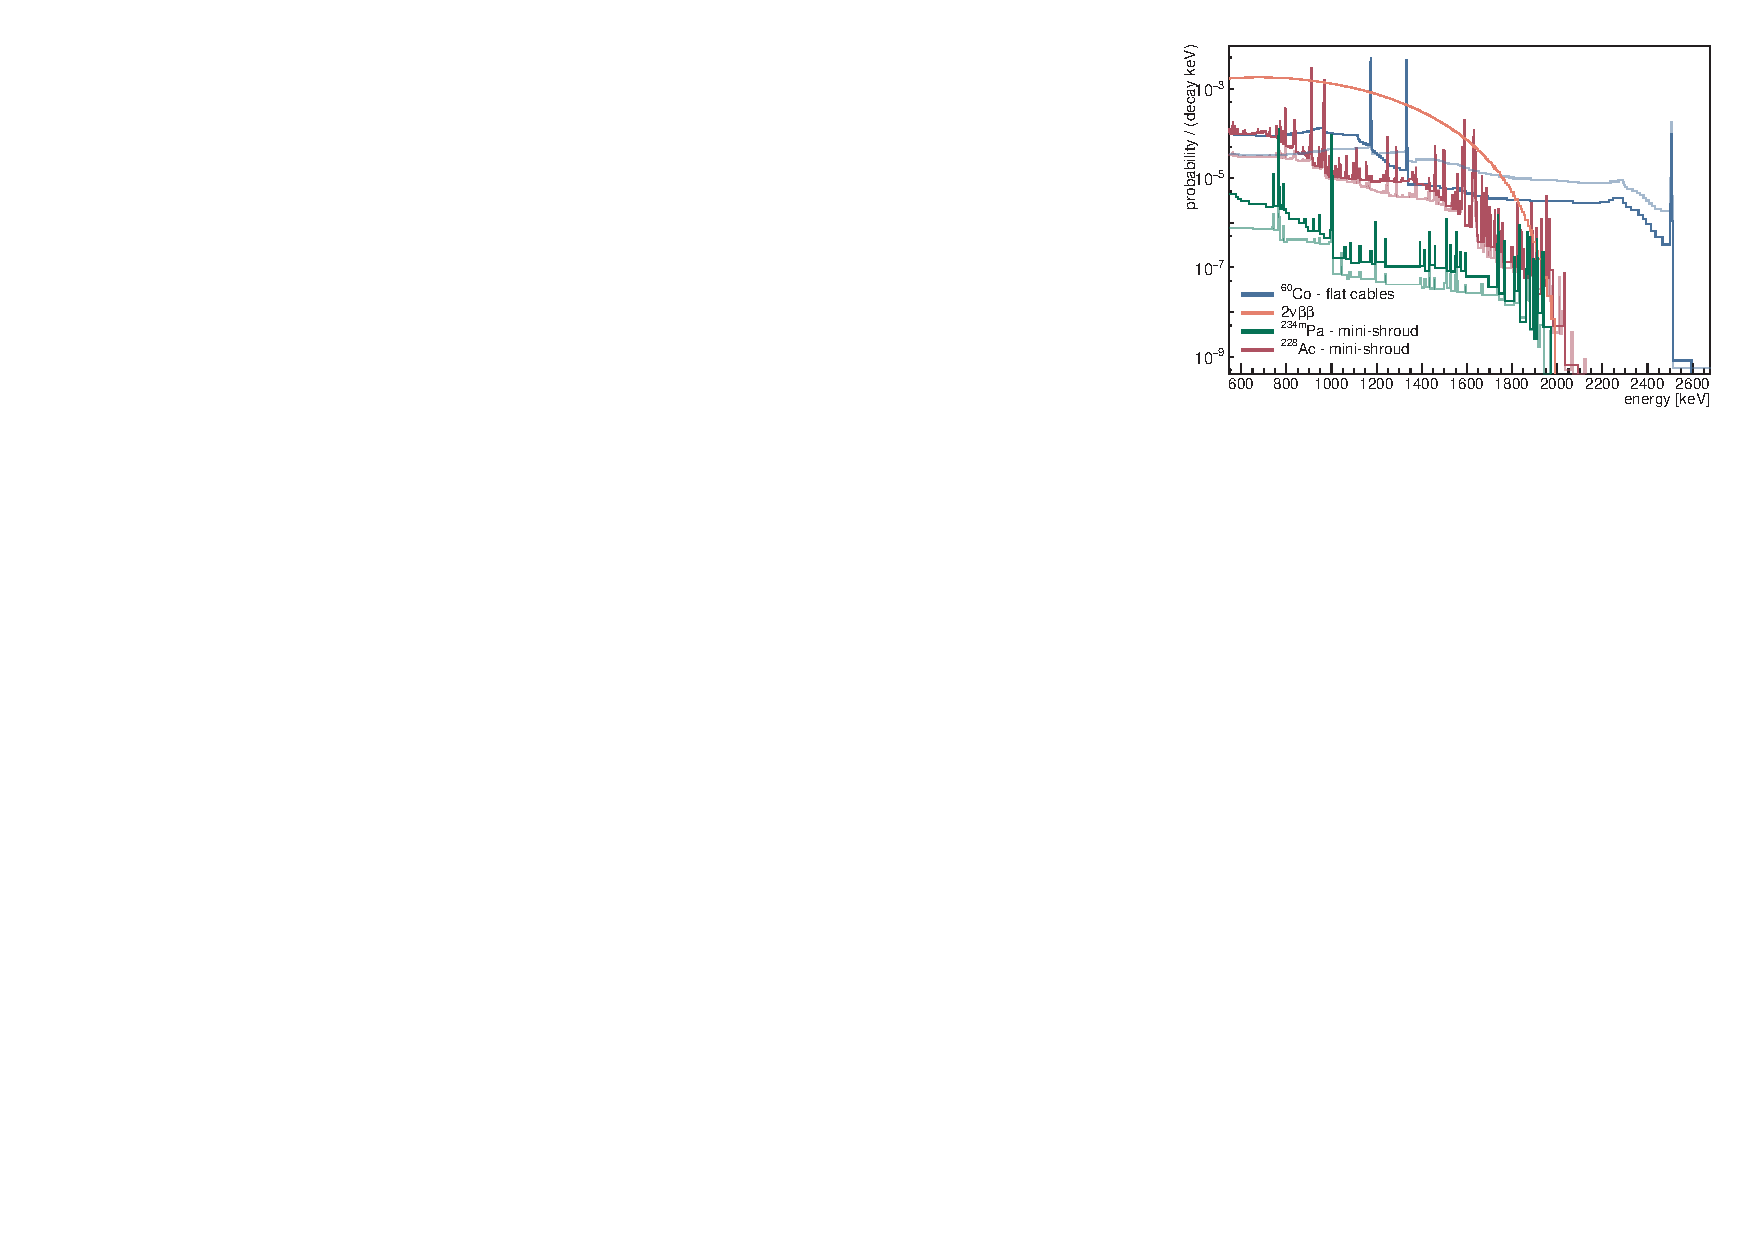
\includegraphics[width=0.45\textwidth]{plots/bkg/raw/ph2/pdfs/gmodel-pdfs-misc.pdf}}
  \hspace{10pt}
  \subfloat[%
    \Bil\ and \Tl\ (\Thh\ chain) contaminations far from (fiber shroud)
    and close to (mini-shrouds) the detector
    array.\label{fig:bkg:raw:ph2:pdfs:gmodel:Th}%
  ]{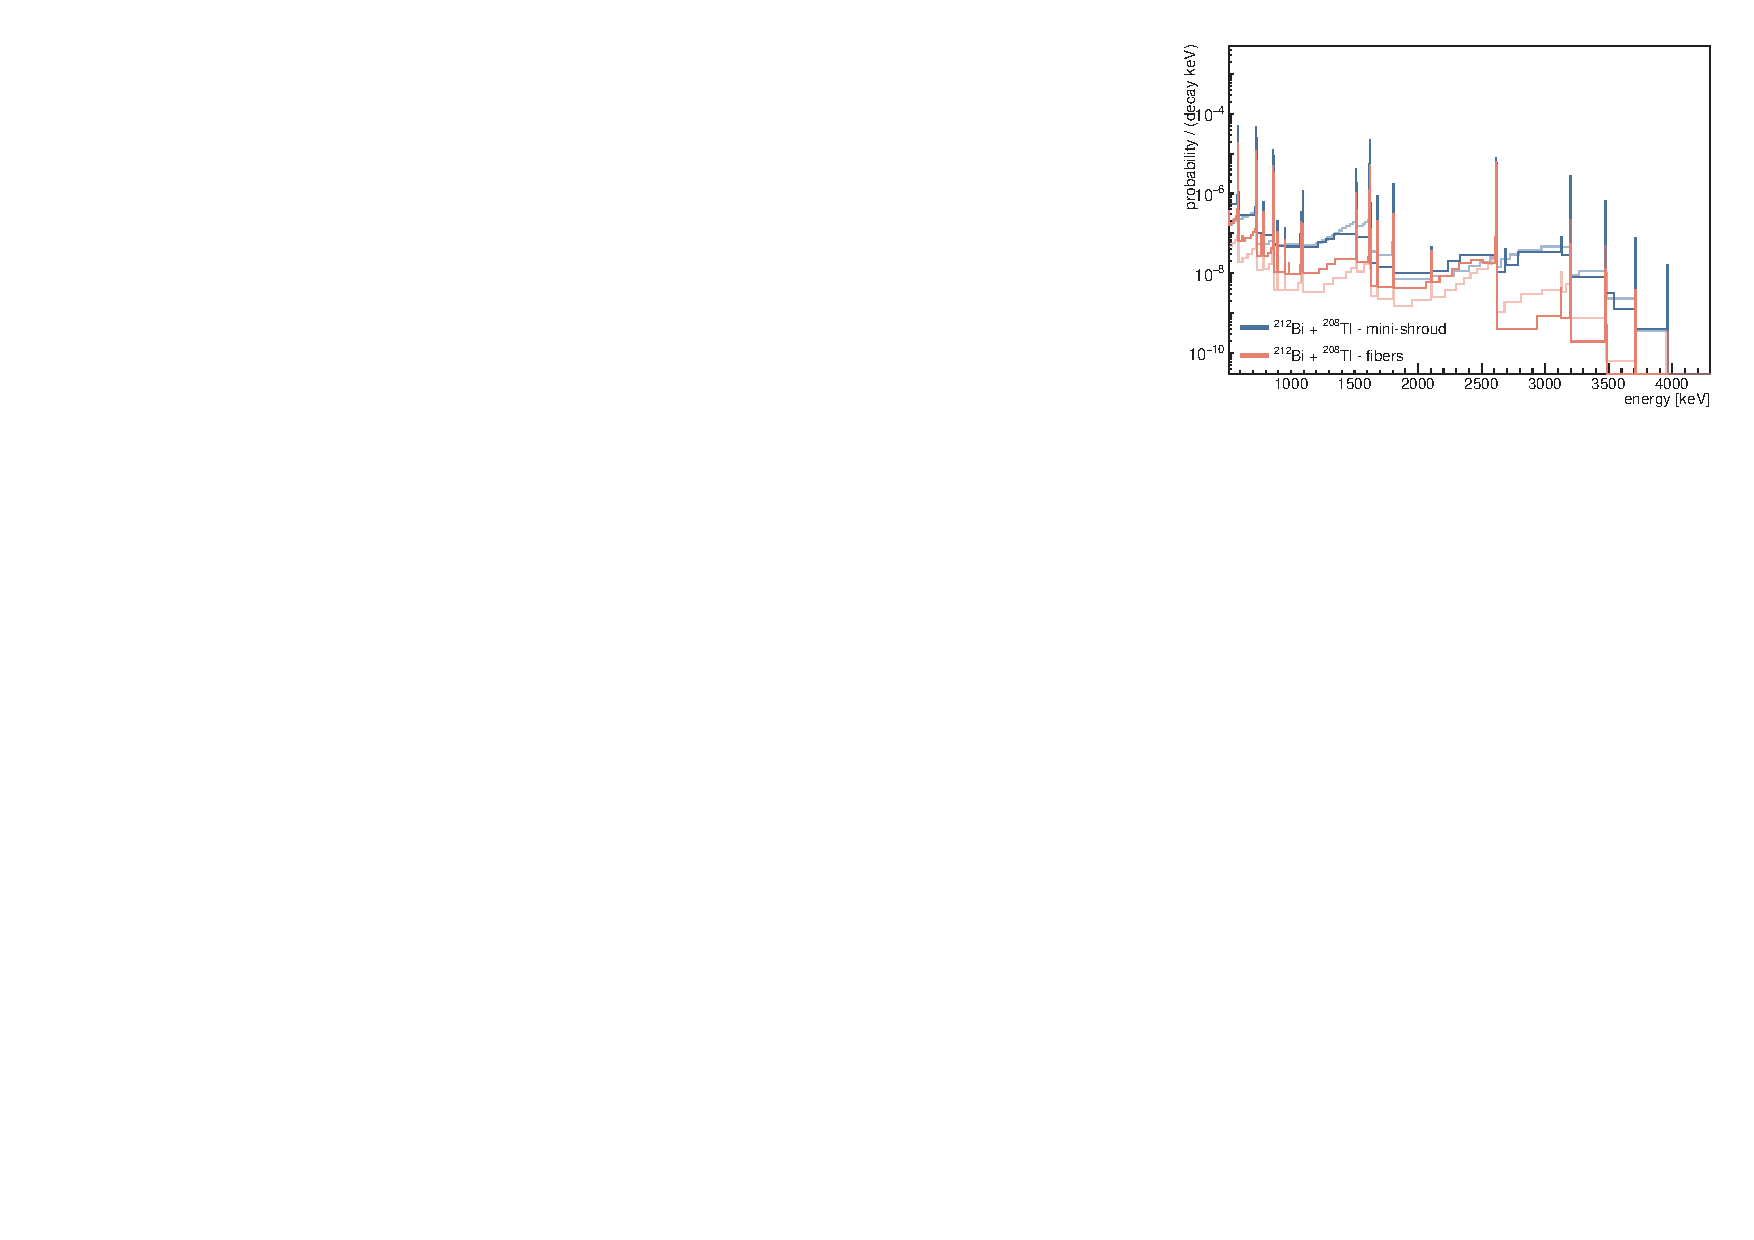
\includegraphics[width=0.45\textwidth]{plots/bkg/raw/ph2/pdfs/gmodel-pdfs-Th.pdf}} \\
  \subfloat[%
    \kvn\ contamination close to the detector array (on the
    mini-shrouds), at a higher radial distance (on the fiber shroud) and
    higher vertical distance (on the copper
    shrouds).\label{fig:bkg:raw:ph2:pdfs:gmodel:K40}%
  ]{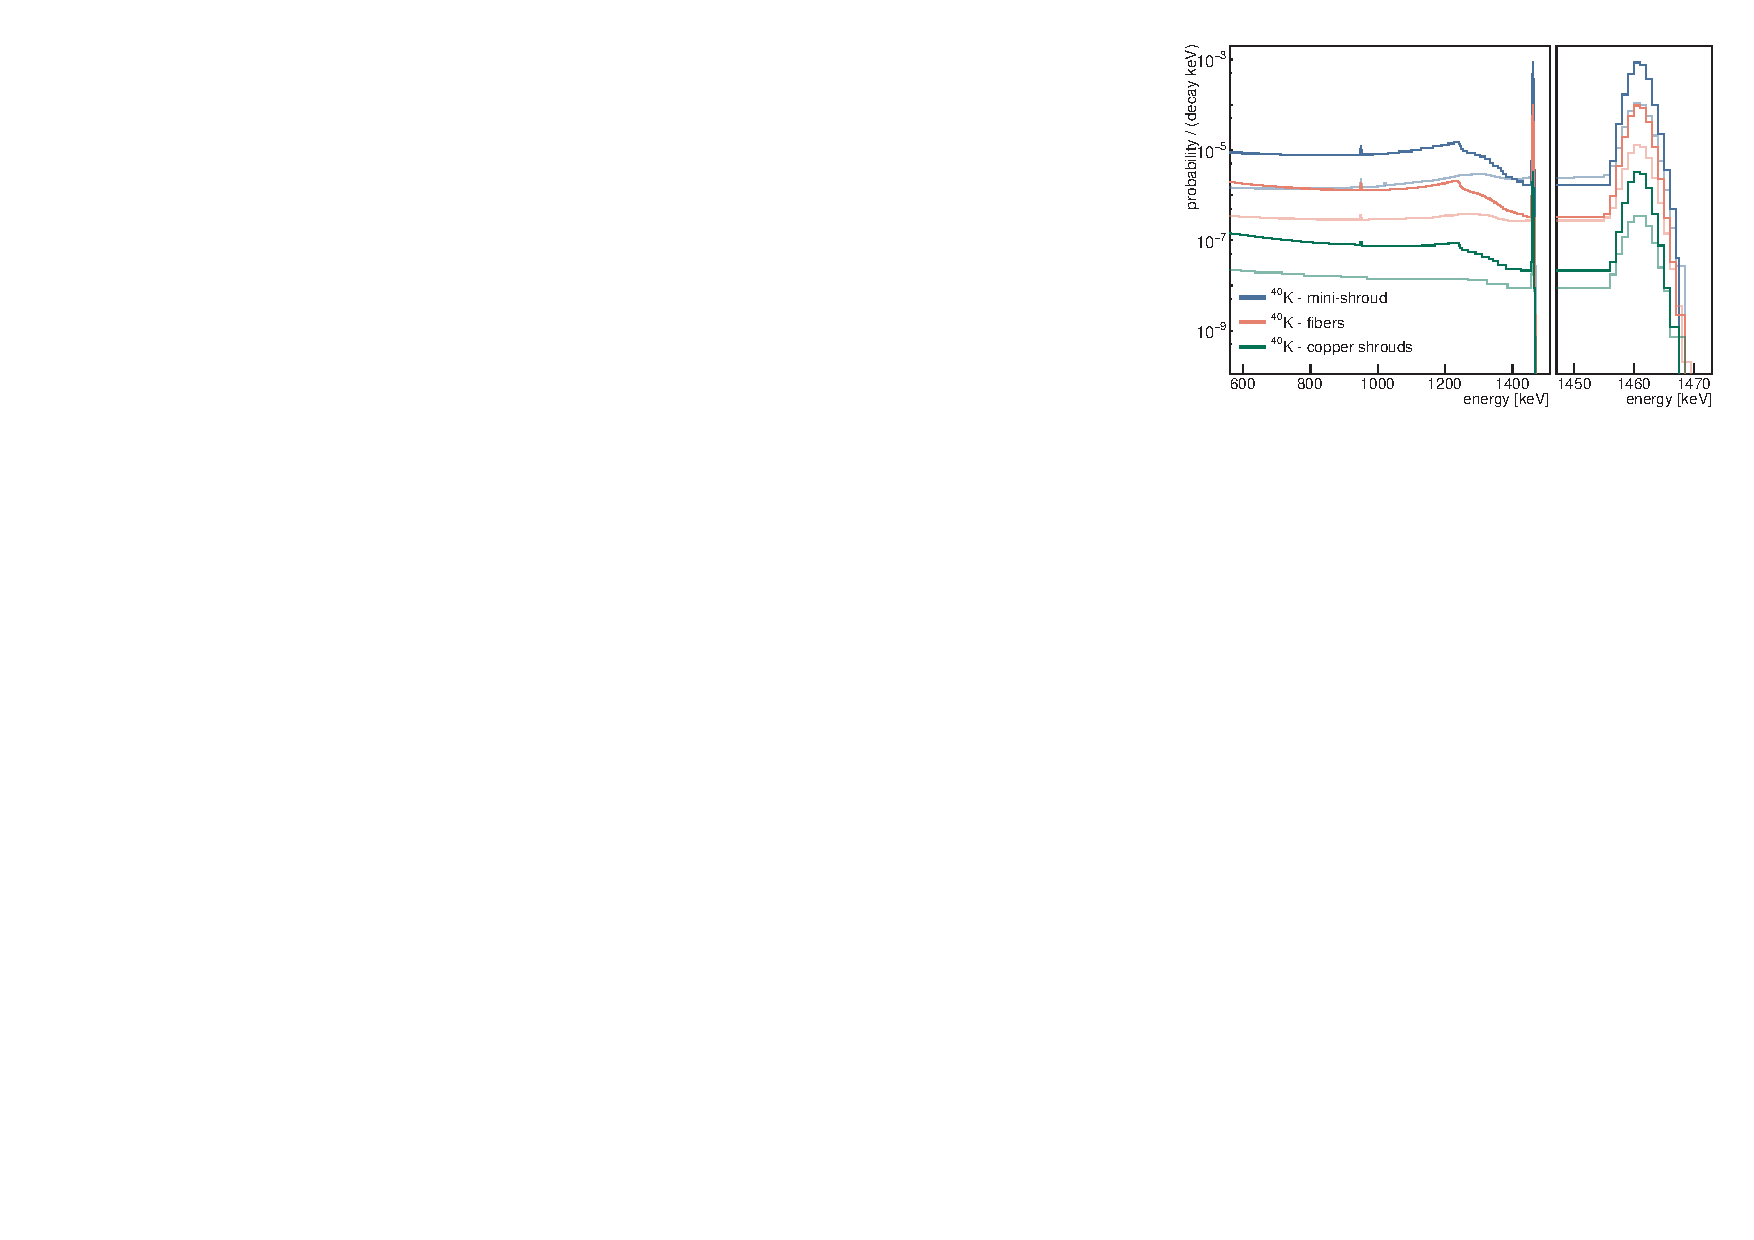
\includegraphics[width=0.45\textwidth]{plots/bkg/raw/ph2/pdfs/gmodel-pdfs-K40.pdf}}
  \hspace{10pt}
  \subfloat[%
    \kvz\ contamination in different locations inside the
    LAr.\label{fig:bkg:raw:ph2:pdfs:gmodel:K42}%
  ]{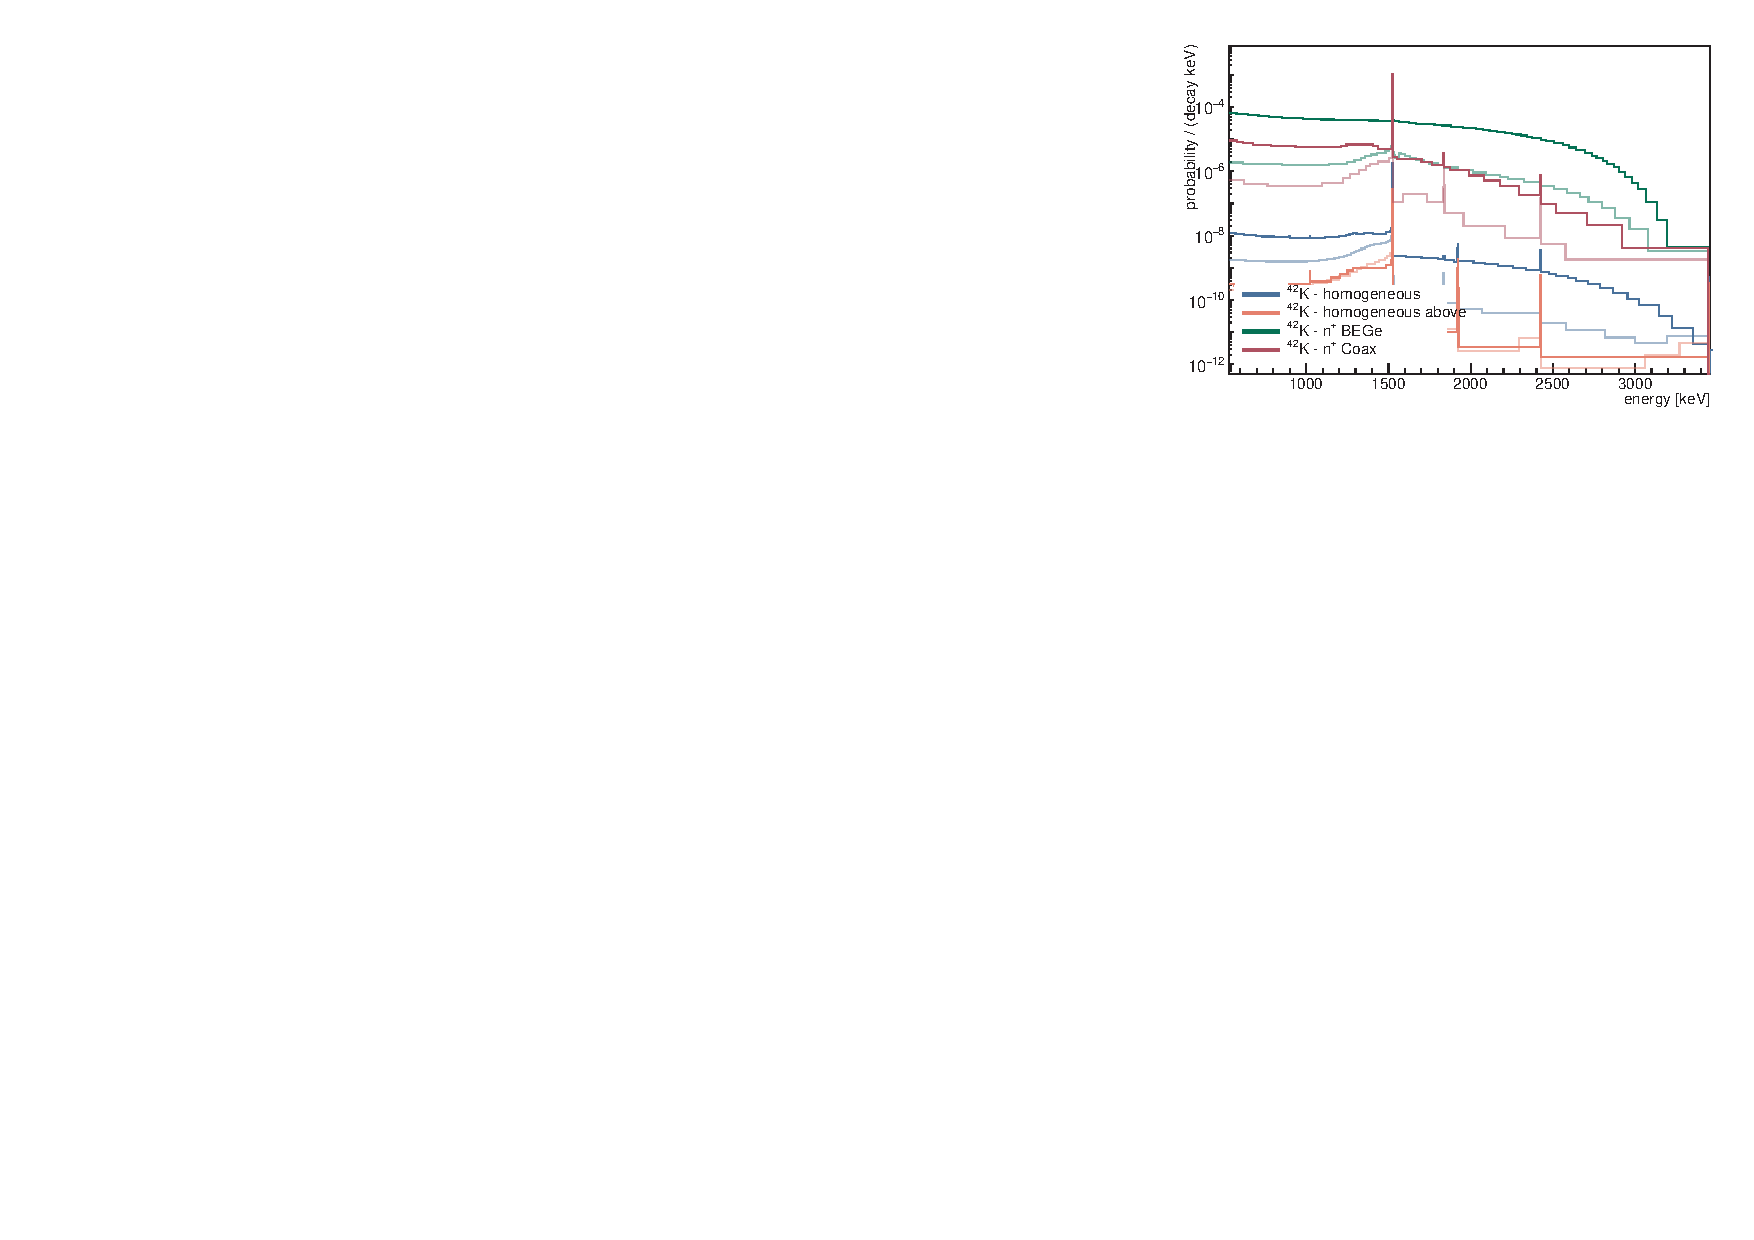
\includegraphics[width=0.45\textwidth]{plots/bkg/raw/ph2/pdfs/gmodel-pdfs-K42.pdf}} \\
  \subfloat[%
    \Po\ \a\ decays on \pplus\ contact surface for different
    thicknesses of the inactive contact layer. For 0~nm the nuclear
    recoil energy can be absorbed and some energy can be lost in the
    LAr.\label{fig:bkg:raw:ph2:pdfs:amodel:Po}%
  ]{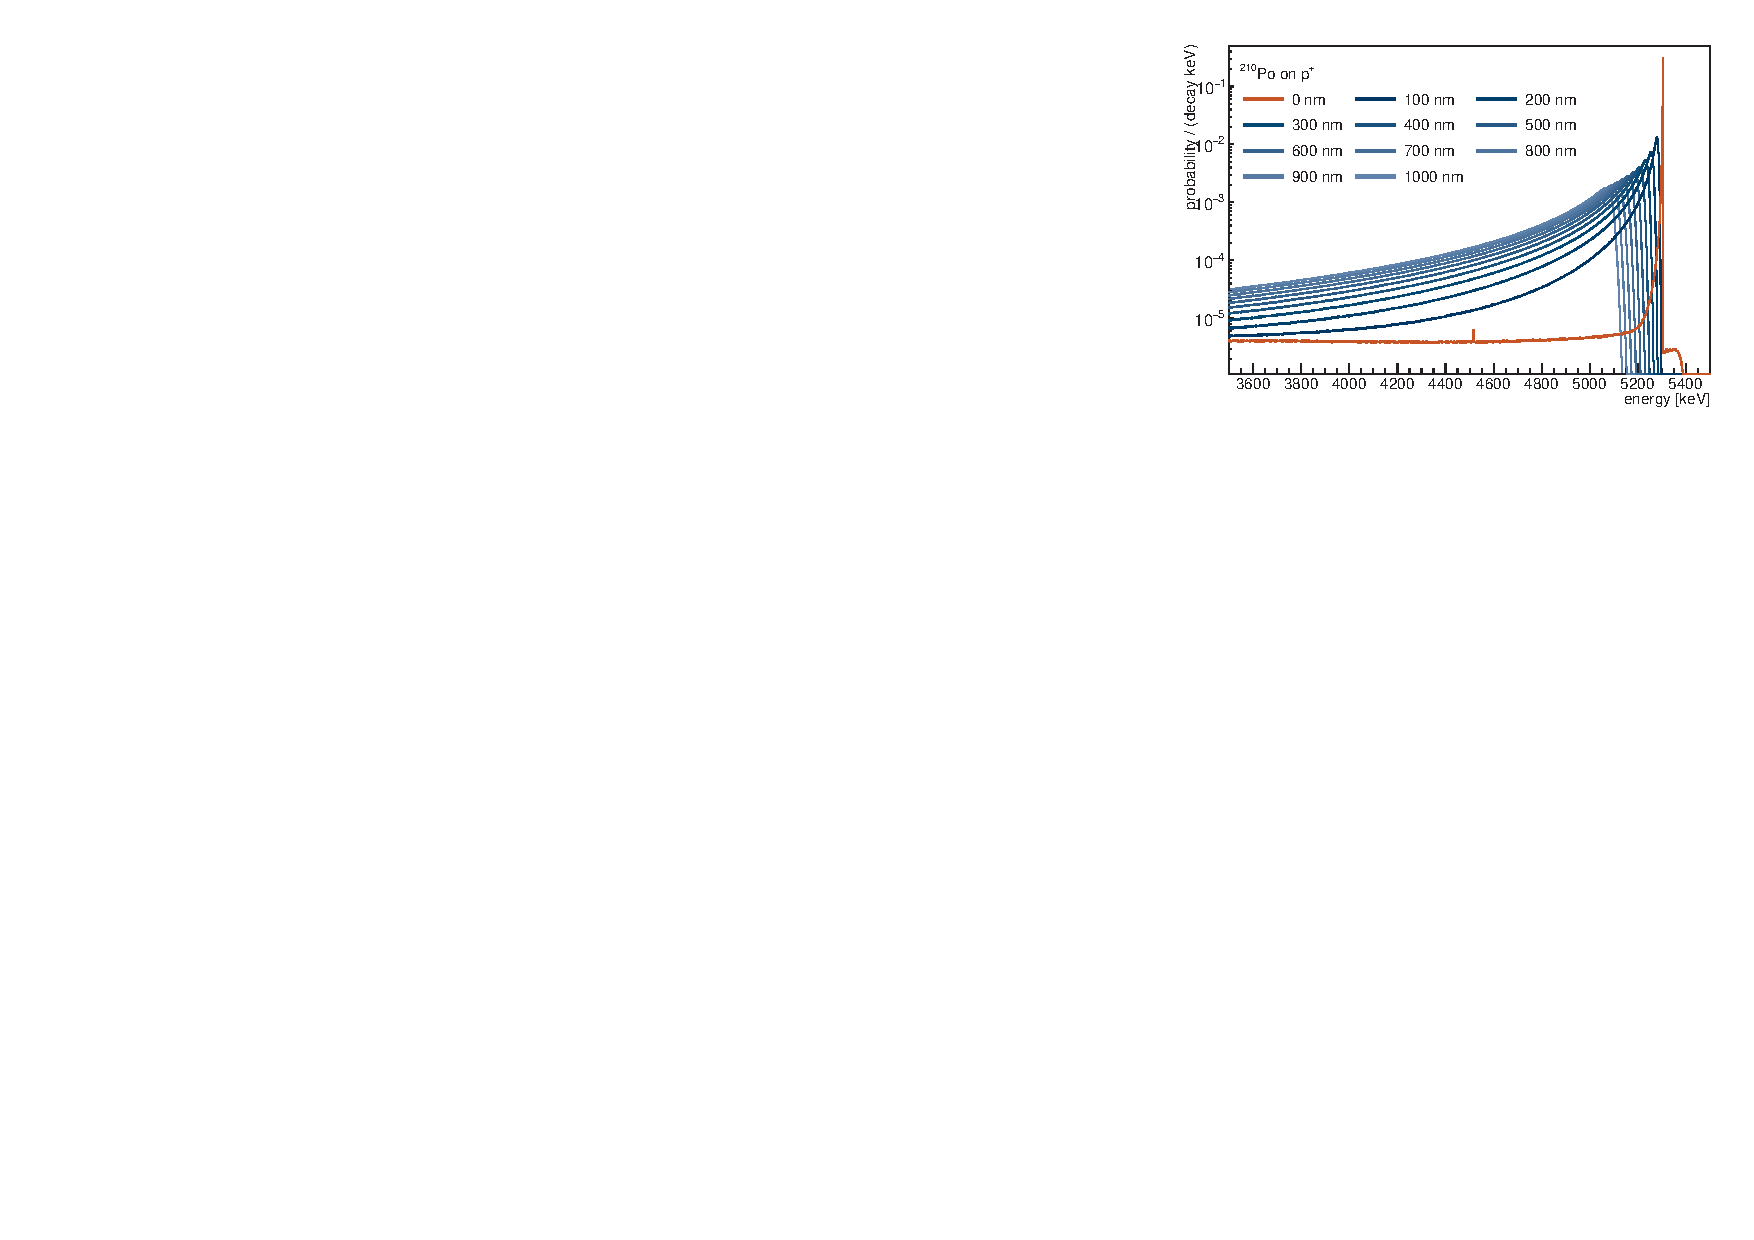
\includegraphics[width=0.45\textwidth]{plots/bkg/raw/ph2/pdfs/amodel-pdfs-Po210.pdf}}
  \hspace{10pt}
  \subfloat[%
    \kvz\ contamination in different volumes in the LAr and detector
    intrinsic \nnbb\ for comparison. The energy window (ROI) considered
    is \mbox{$(1525\pm4)$~keV} (\kvz\ \g\ line).\label{fig:bkg:raw:ph2:pdfs:kmodel:K42}%
  ]{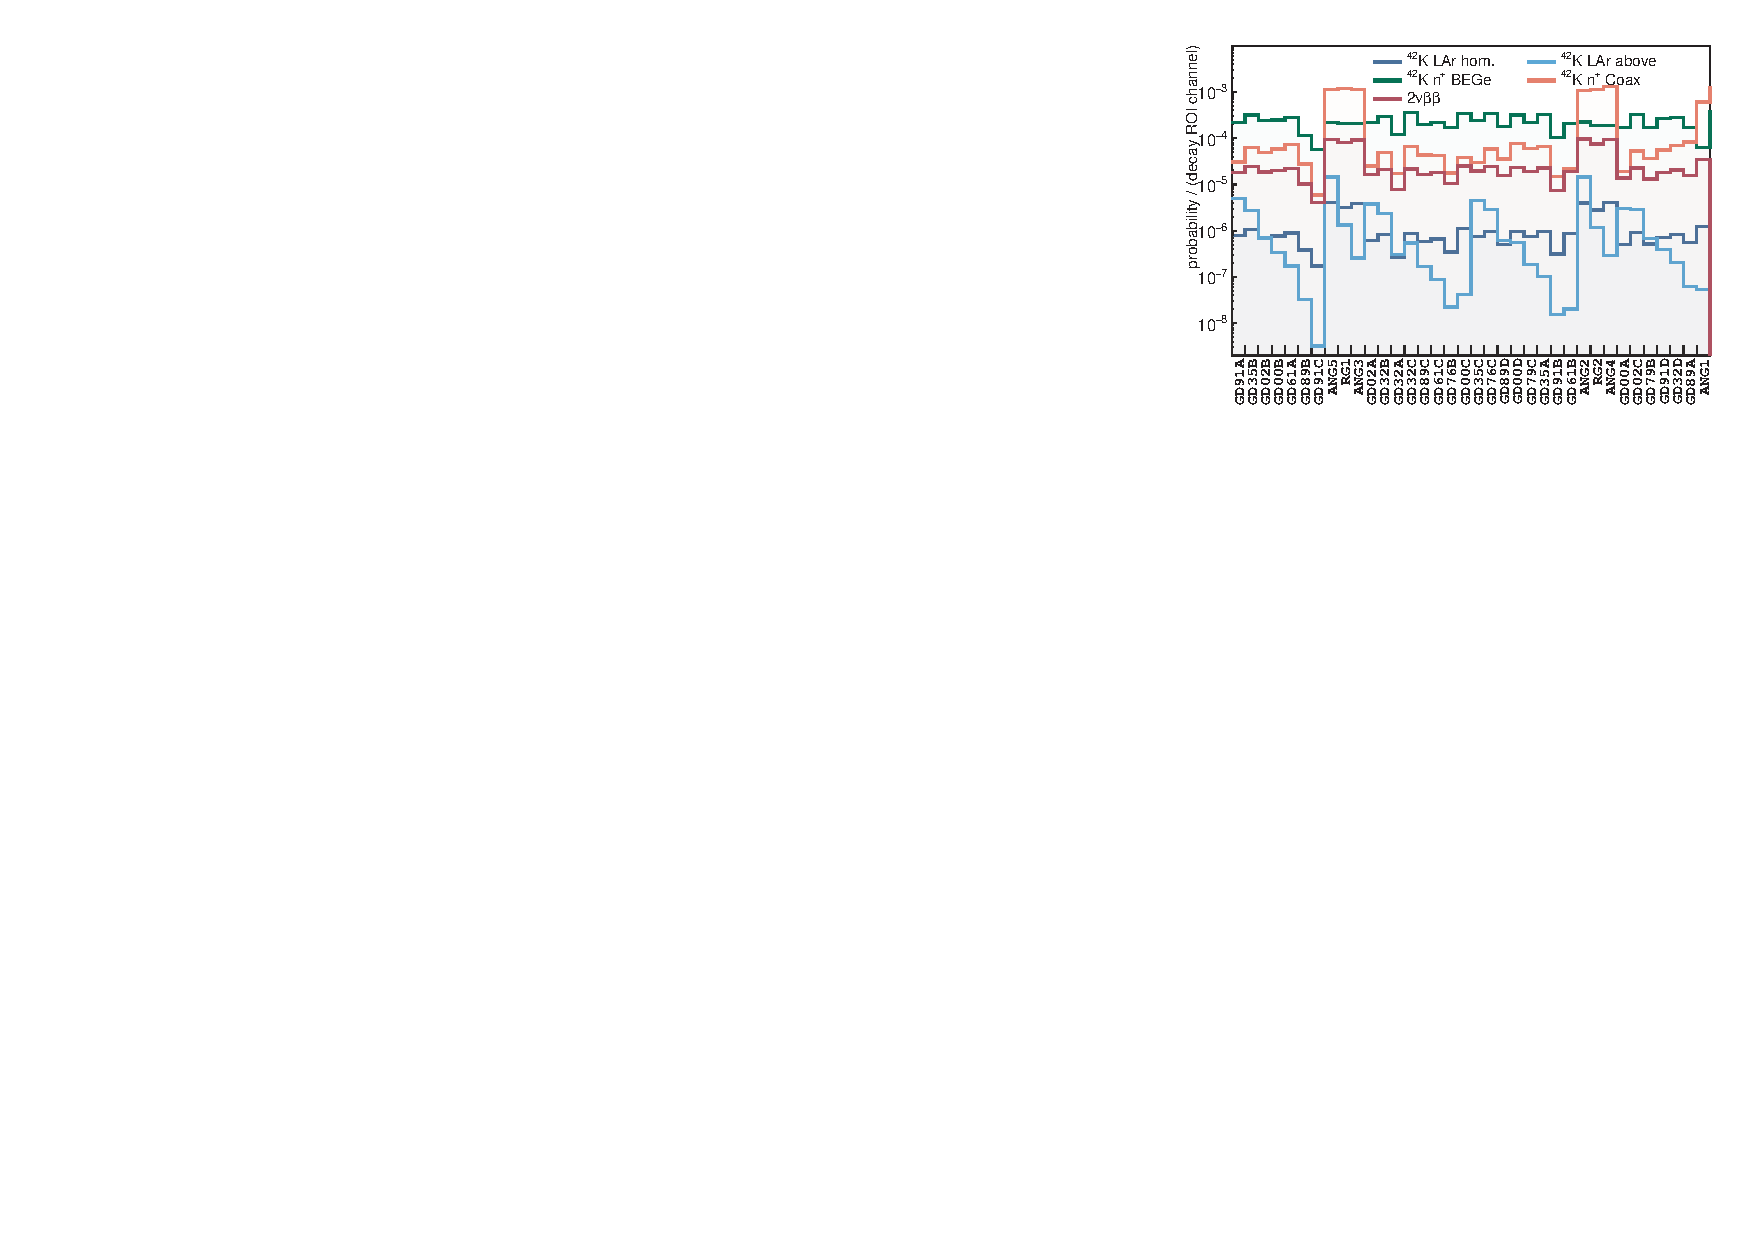
\includegraphics[width=0.45\textwidth]{plots/bkg/raw/ph2/pdfs/kmodel-pdfs-K42-long.pdf}}

  \caption{%
    From (a) to (e): pdfs in the full energy domain. The pdfs for the
    \enrGeII\ ($\enrBEGeII + \enrCoaxII$) (in fully opaque colors)
    and the \enrGeII\ (in shaded colors) data sets relative to different
    background sources. For visualization purposes a variable binning is
    adopted. (f) pdfs per detector channel for the \kvz\ \g\ line.
    All pdfs are normalized to the number of simulated primary decays.
  }\label{fig:bkg:raw:ph2:pdfs:gmodel}
\end{figure}

\section{Statistical Analysis}%
\label{sec:bkg:raw:ph2:stat}

The multivariate statistical analysis, which is used to model and disentangle the
background in its components, runs on the three binned data sets \enrBEGeII, \enrCoaxII\
and \enrGeII.The single-detector data sets \enrBEGeII\ and \enrCoaxII\ contain the
reconstructed energy of all \Mone\ events whereas for the two-detector events the sum of
the two reconstructed energies is put in the \enrGeII\ data set. Moreover, the count rate
per detector is used for the two potassium \g\ lines.  The spatial event distribution is a
collection of the number of events per detector for \Mone\ events and expressed in a
matrix of pairs of detectors for all \Mtwo\ events.

Assuming that the number of events in each bin follows the Poisson probability
distribution $\text{Pois}(n;\nu)$, where $\nu$ is the expected mean and $n$ is the
experimentally measured number of counts, the likelihood function for a binned data set
reads $\prod_{i=1}^{N_\text{bins}} \text{Pois}(n_i;\nu_i)$. Here $\nu_i =
\sum_{k=1}^{N_\text{com}} \nu_i^{(k)}$ is the expected number of events in the $i$-th bin,
calculated as the sum of the contributions from each background component $k$;
$\nu_i(\lambda_1, \ldots, \lambda_{N_\text{com}})$ is a function of the parameters of
interests $\lambda_j$ (isotope activities, \nnbb\ half-life, etc.). The complete
likelihood function adopted for the present analysis combines the three data sets
\enrBEGeII, \enrCoaxII\ and \enrGeII:
\begin{equation}\label{eq:bkg:raw:ph2:likelihood}
  \mathcal{L}(\lambda_1, \ldots, \lambda_m \,|\, \text{data}) =
    \prod_{d=1}^{N_\text{dat}}
    \prod_{i=1}^{N_\text{bins}}
    \text{Pois}(n_{d,i};\nu_{d,i})\;.
\end{equation}

The statistical inference is made within a Bayesian framework. Hence, to obtain posterior
probabilities for the free parameters of interest $\lambda_j$, the likelihood defined in
\cref{eq:bkg:raw:ph2:likelihood} is multiplied according to the Bayes theorem by a factor
modeling the prior knowledge of each background component as presented in
\cref{sec:bkg:raw:ph2:priors}. The computation is performed using a Markov Chain Monte
Carlo (MCMC) and is implemented using the BAT software suite~\cite{Caldwell2008,
Beaujean2018}. Posterior probability distributions of any observable that is not a free
parameter of the likelihood function, like background index estimates, are obtained by
sampling the desired parameter from the MCMC. A \pvalue\ estimate is provided as a
goodness-of-fit measure by adopting the algorithm suggested in~\cite{Beaujean2011} for
Poisson-distributed data.  It has to be kept in mind that this \pvalue\ estimate, however,
is not as well suited for model comparison as is for instance a Bayes factor; e.g.~the
number of free parameters is not taken into account while a Bayes factor always penalizes
models that add extra complexity without being required by the data.

\subsection{Analysis window and binning}

The fit range and data bins are chosen such as to exploit as much information from
spectral features as possible brought by data without introducing undesired bias. The
chosen fit range in energy space for the single-detector data sets (\enrBEGeII\ and
\enrCoaxII) starts from just above the end-point of the \Arl\ $\beta^-$-spectrum at
565~keV and ends just above the \Po\ peak at 5260~keV, where the event rate drops to
almost zero values. For the two-detector events (\enrGeII\ data set) the fit range starts
at 520~keV and extends up to 3500~keV. Possible additional components outside of this
range (e.g. \Arl) do neither add information to the background decomposition in the ROI
around \qbb\ nor to the analysis of \nnbb\ decay. Furthermore, at energies lower than
$\sim$100~keV the shape of the pdfs is dominated by uncertainties on the detector
transition layer model, which describes the charge-carrier collection at the interface
between the \nplus\ contact and the detector active volume. The exact nature of this
transition region is different for each detector and prone to systematic
uncertainties~\cite{Lehnert2016}.

With an energy resolution which is typically 3--4~keV at \qbb\ (FWHM)~\cite{Agostini2018,
Agostini2019a} and better at lower energies, a fixed bin size of 1~keV was chosen for all
data sets. The only exceptions are the two \g\ lines from \kvn\ and \kvz\ each of which is
combined in a single bin from 1455~keV to 1465~keV and from 1520~keV to 1530~keV,
respectively. This is done in order to suppress any systematic uncertainties of the energy
calibration and resolution model that affect the position and shape of the \g\
lines~\cite{Agostini2019}.

\subsection{Likelihood factorization}%
\label{sec:bkg:raw:ph2:likelihoodfact}

A feature of the selected data is that the likelihood in
\cref{eq:bkg:raw:ph2:likelihood} can be factorized in uncorrelated parts which can be
studied individually and in detail. In the following we shortly outline the parts of the
data which were studied in depth based on the approach of factorizing the likelihood into
uncorrelated parts. Finally, the results of these analyses are incorporated into a
full-range fit. This procedure is equivalent to a simultaneous analysis of all data but
increases the input knowledge for the fit and breaks down the computational complexity in
smaller steps.

\blocktitle{Potassium \\ tracking \\ analysis}
As can be noted from \cref{fig:bkg:raw:ph2:pdfs:gmodel:K40} and
\cref{fig:bkg:raw:ph2:gmodel:K42} the pdfs of \kvn\ and \kvz\ in energy are prone to
degeneracies and hence parameter correlations. Their most prominent \g\ lines at 1461~and
1525~keV, respectively, contain information on the spatial distribution while the
two-detector events contain information about the angular distribution of Compton
scattered events. Their combination is beneficial in order to pin down the potential
location of the two potassium isotopes. In total the \texttt{M1} data contains 4472~cts in
$1461\pm4$~keV and 6718~cts in $1525\pm4$~keV while the \texttt{M2} events contain 554~cts
in $1461\pm6$~keV and 865~cts in $1525\pm6$~keV, respectively. An analysis of the number
of events in the two potassium \g\ lines in each detector (and detector pair) is used to
exploit mainly top-down and rotational asymmetries in the \kvn\ and \kvz\ distributions.
The number of events in the two energy windows are summarized detector-by-detector; in the
following we refer to this procedure as \textit{projection in detector space}. The
treatment of the likelihood in \cref{eq:bkg:raw:ph2:likelihood} is outlined in detail in
\cref{apdx:kmodel}.  The number of events in all other \g\ lines is too low in order to
adopt a useful detector-wise analysis. The spatial analysis of \kvn\ and \kvz\ is
incorporated in the full-range fit by directly employing the posterior parameter
distributions as prior information.\footnote{By adopting this approach, a part of the data
in the potassium \g\ lines region is analyzed twice: first in the potassium tracking
analysis and then in the full-range fit. Nevertheless, considering that the two analyses
exploit different data features (i.e.~count rate per detector and total count rate per
energy) and the overlap between the two data set is minimal, the overall effect is
negligible.}

\blocktitle{\a\ events background analysis}
The single-detector energy spectra above 3.5~MeV (the Q-value of \kvz\ \b\ decay) are
strongly dominated by \a\ events. They are not present in two-detector data due to the
short range of \a\ particles in LAr and germanium. Also, this component is not correlated
to other backgrounds considered here because it peaks at energies well above the highest
\g\ emission energies and \b\ decay Q-values. A careful study was carried out considering
various \pplus\ contact thickness and event rates to reproduce the \Po\ peak. In order to
reproduce \a\ events with degraded energy an empirical model is fit to the data. A linear
function with free slope and offset and a cut-off below the maximum of the \Po\ peak fits
the data well. The agreement of the \a\ background model with the data is demonstrated in
\cref{apdx:amodel} and \cref{fig:apdx:alphafit} therein. Information from the detailed
analysis of the high-energy \a\ region is incorporated in the full-range fit using a
combined pdf that summarizes the \Po\ peak plus the \Ra\ decay chain and a linear floating
component for degraded \a\ events.

\subsection{Prior distributions}

The following criteria are adopted to convert the prior information described in
\cref{sec:bkg:raw:ph2:priors} into prior probability distributions on the parameters of
interest\footnote{In Bayesian analysis the prior probability distribution describes all
knowledge about an unobserved quantity of ultimate interest before taking the data into
account.}: if a measured value with uncertainty is available for a background
contamination then a Gaussian distribution with a corresponding centroid and a $1\sigma$
width is adopted. In presence of a 90\% C.L.~upper limit, instead, an exponential prior
distribution is constructed with 90\% of its area covering parameter values from 0 up to
the given 90\% C.L.~upper limit. A uniform prior distribution is assigned to components
for which no measured value or upper limit is available. Ranges for uniform priors are
initially taken very wide, in order to span a large portion of the allowed parameter
space, then optimized to contain at least 99\% of the posterior distribution. As mentioned
before, in addition to the information from screening measurements, prior distributions
for \kvn\ and \kvz\ are constructed considering the posterior inference from their spatial
distribution.\footnote{The Bayesian posterior distribution is the conditional probability
distribution of the unobserved quantities of ultimate interest, given the observed
data.} Moreover, as \Bih\ is part of the \Ra\ decay chain, we constrain a \Bih\ component
on the \pplus\ contact by a Gaussian prior extracted from the obtained \Ra\ activity based
on the energy estimator in the high-energy \a\ region.

\section{\texorpdfstring{\a\ events analysis}{alpha events analysis}}%
\label{sec:bkg:raw:ph2:amodel}

Above an energy of 3.5~MeV almost all registered events are due to \a-emitting isotopes.
The respective part of the full likelihood can be approximately factorized and studied
separately.  \a\ particles have a very short range in LAr as well as in germanium
(continuous slowing down approximation, CSDA, range of 50~\mum\ and 20~\mum,
respectively~\cite{Berger2017} and are able to reach a detector's active volume only
through the very thin (of the order of 500~nm) \pplus\ contact surface. Therefore, the \a\
emitter contamination is detector-specific and depends only on the \pplus\ surface
contaminations. Therefore, we analyze the \enrBEGeII\ and \enrCoaxII\ detector data
separately in energy space; the projection in detector space bares no correlation between
detectors and hence contains no further useful information. The number of events in a
single detector is not sufficient to further split the data on a detector-by-detector
basis. The two data sets are uncorrelated and the statistical analysis can be carried out
for each single-detector data set separately. In the two-detector data the \a\ component
is not observed due to the short range of these particles.

All contaminations found are constituents of the \Uh\ decay chain. The main surface
contamination observed is \Po\ which occurs either as an incident contamination and decays
in time with a half-life of $138.3763(17)$~days~\cite{Be2008} or is fed by a contamination
with \Pbl\ with a stable rate in time. The spectral form is identical for both cases and
can only be disentangled by analyzing the \a-event rate in time.

Above the \Po\ peak very few events are observed. In the \enrBEGeII\ data set we find only
four events with an energy larger than 5.3~MeV, while in the \enrCoaxII\ data set 22 such
events are observed, 14 of which in a single detector \ANG{2}
(see~\cref{tab:bkg:raw:ph2:amodel:rncts}). These events are due to \a\ decays from \Rn\
and subsequent isotopes on the \pplus\ detector surfaces. \ANG{2} also shows a higher \Ra\
(mother nucleus of \Rn) contamination which suggests dominantly a surface contamination
with \Ra\ rather than \Rn\ dissolved in the LAr. In the latter case the decay chain would
be broken as only the gaseous \Rn\ emanates from the construction materials into the LAr.
Unfortunately, the number of counts is too low to distinguish the spectral shape above
5.3~MeV and disentangle a surface contamination with \Ra\ from \Rn\ dissolved in LAr. A
comparison between the counts observed above 5.3~Mev and the \Bih\ 609~keV \g\ line
suggests that \a\ events due to a dissolved \Rn\ contamination would not produce
observable counts in said energy region. Assuming that all \Bih\ observed comes from
dissolved \Rn\ leads, in fact, to a specific activity smaller than 10~\mubq/kg. Hence, in
the following, we will only consider a \pplus\ surface contamination with \Ra\ and all
subsequent isotopes to which we refer as the \Ra\ decay chain. The \Po\ and \Ra\
contaminations are not necessarily spatially correlated.
\begin{table}
  \centering
  \caption{%
    Observed number of counts with energy >5.3~MeV belonging to
    the \Ra\ decay chain. Detectors with zero counts are not listed.
  }\label{tab:bkg:raw:ph2:amodel:rncts}
  \begin{tabular}{cccc}
    \toprule
    data set                    & detector & channel & \Ra\ chain [cts] \\
    \midrule
    \multirow{3}{*}{\enrBEGeII} & \GD{61C} & 16      & 1                \\
                                & \GD{79B} & 32      & 1                \\
                                & \GD{89A} & 35      & 2                \\
    \midrule
    \multirow{6}{*}{\enrCoaxII} & \ANG{1}  & 36      & 2                \\
                                & \ANG{2}  & 27      & 14               \\
                                & \ANG{3}  & 10      & 1                \\
                                & \ANG{4}  & 29      & 1                \\
                                & \ANG{5}  &  8      & 2                \\
                                & \RG{1}   &  9      & 2                \\
    \bottomrule
  \end{tabular}
\end{table}

Due to the very short range of \a\ particles the energy spectrum of \a\ decays exhibits a
line with a pronounced low-energy tail. The tail is formed when the decay occurs under an
incident angle with respect to the contact and the \a\ particle loses part of its energy
before reaching the detectors active volume. The maximum is shifted with respect to the
full emission energy which is due to energy loss inside the electrode and depends on its
minimal thickness. The detectors have slightly different contact thicknesses, also, the
\pplus\ contact of a single detector may intrinsically be inhomogeneous.  Therefore, we
model the \Po\ peak with a mixture of pdfs obtained from simulations with different
contact thicknesses. Due to the low number of counts observed in the \Ra\ chain it is
sufficient to model this component with only one pdf. Furthermore, the isotope
contamination is assumed to halve at each decay step. A reduction effect of the subsequent
\a\ decays in the \Rn\ chain had been observed in \phaseone\ and attributed to possible
recoil off the surface into the LAr~\cite{Agostini2013}. We adopt this explanation in our
model although we note that the number of events observed with an energy >5.3~MeV is not
sufficient to confirm the previously observed reduction effect.  Further details about the
construction of the pdfs are given in \cref{apdx:magepdfs}.

Dedicated measurements~\cite{Agostini2013b} have shown that events originating in the
contact separating groove are partly reconstructed with degraded energy. A
simulation-based model of these energy-degraded events is not available yet. We
approximate this component with an empirical linear distribution truncated below the
maximum of the \Po\ peak. Such a component accommodates also eventual \a\ decays in the
LAr in very close vicinity to the \pplus\ detector surface. However, the number of events
found with an energy >5.3~MeV is too low to fully account for the linearly modeled
distribution.

The likelihood function for modeling the high-energy region dominated by \a\ decays runs
only on single-detector data, namely \enrBEGeII\ and \enrCoaxII\ separately, in a range
from 3.5~MeV to 5.25~MeV. Events with an energy higher than 5.25~MeV are put in a single
overflow bin:
\begin{equation}
  \mathcal{L}_\alpha(\lambda_1,\ldots,\lambda_m\,|\,n) =
  \prod_{i=1}^{N_\text{bins}} \text{Pois}(n_{i};\nu_{i})\;
  \label{eq:bkg:raw:ph2:amodel:likelihood}
\end{equation}
A flat prior probability is assigned to each of the fit parameters $\lambda_i$. Both data
sets are fit separately with a fixed bin size of 10~keV\footnote{The calibration curves
are accurate on the sub-keV level up to the highest \g\ energy of about 2.6~MeV emitted
by the \Th\ calibration sources. Although no major non-linearity effects were found the
same accuracy cannot be guaranteed at 6~MeV. Deviations from linearity at this energy are
within 10~keV, hence, we increase the bin size in the higher energy range.} as the \a\
contamination is detector individual and the two single-detector data sets are
uncorrelated in the respective energy window.

The fit results are shown in \cref{fig:bkg:raw:ph2:amodel:resultsplot} and listed in
\cref{tab:bkg:raw:ph2:amodel:results}. The \Po\ component is modeled with a combination of
\pplus\ contact thicknesses from 400 to 600~nm for the \enrBEGeII\ data set and from 300
to 700~nm for the \enrCoaxII\ data set in steps of 100~nm. Further \Po\ components are
rejected by a Bayes factor analysis.  Impurities belonging to the \Ra\ chain are mostly
located on \ANG{2} and thus a fit of the \enrCoaxII\ data set using a single \pplus\
thickness describes this component well. For the \enrBEGeII\ data set we observe a very
small number of counts for the \Ra\ chain, therefore, also in this case a single component
is sufficient. We determine a best-fit value of 100~nm and 500~nm, respectively. The
estimated \pvalue\ for \enrBEGeII\ is 0.2 whereas the \pvalue\ for \enrCoaxII\ is 0.3. The
dominant spectral component below 4.5~MeV is due to degraded \a\ events which extends down
to the ROI.

\begin{figure}
  \centering
  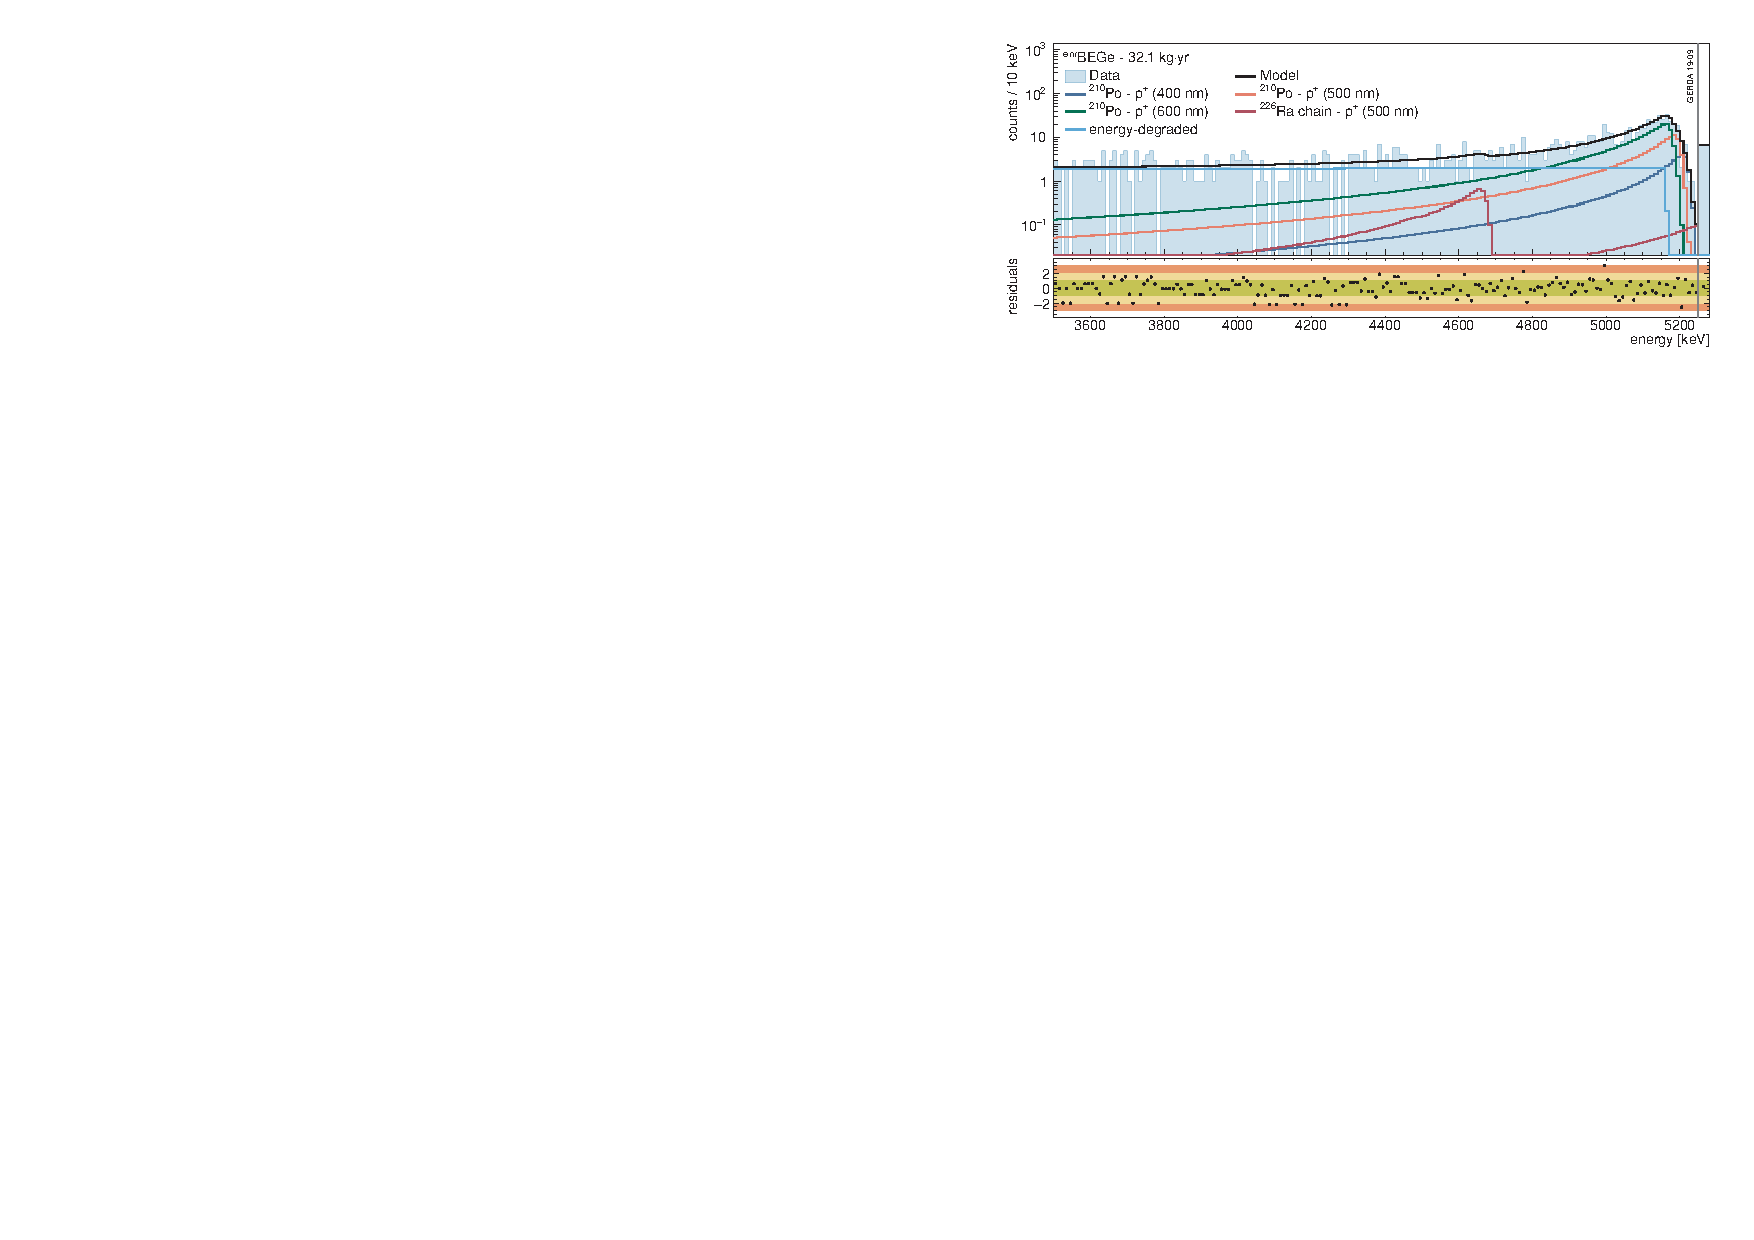
\includegraphics{plots/bkg/raw/ph2/results/amodel/amodel-enrBEGe.pdf}
  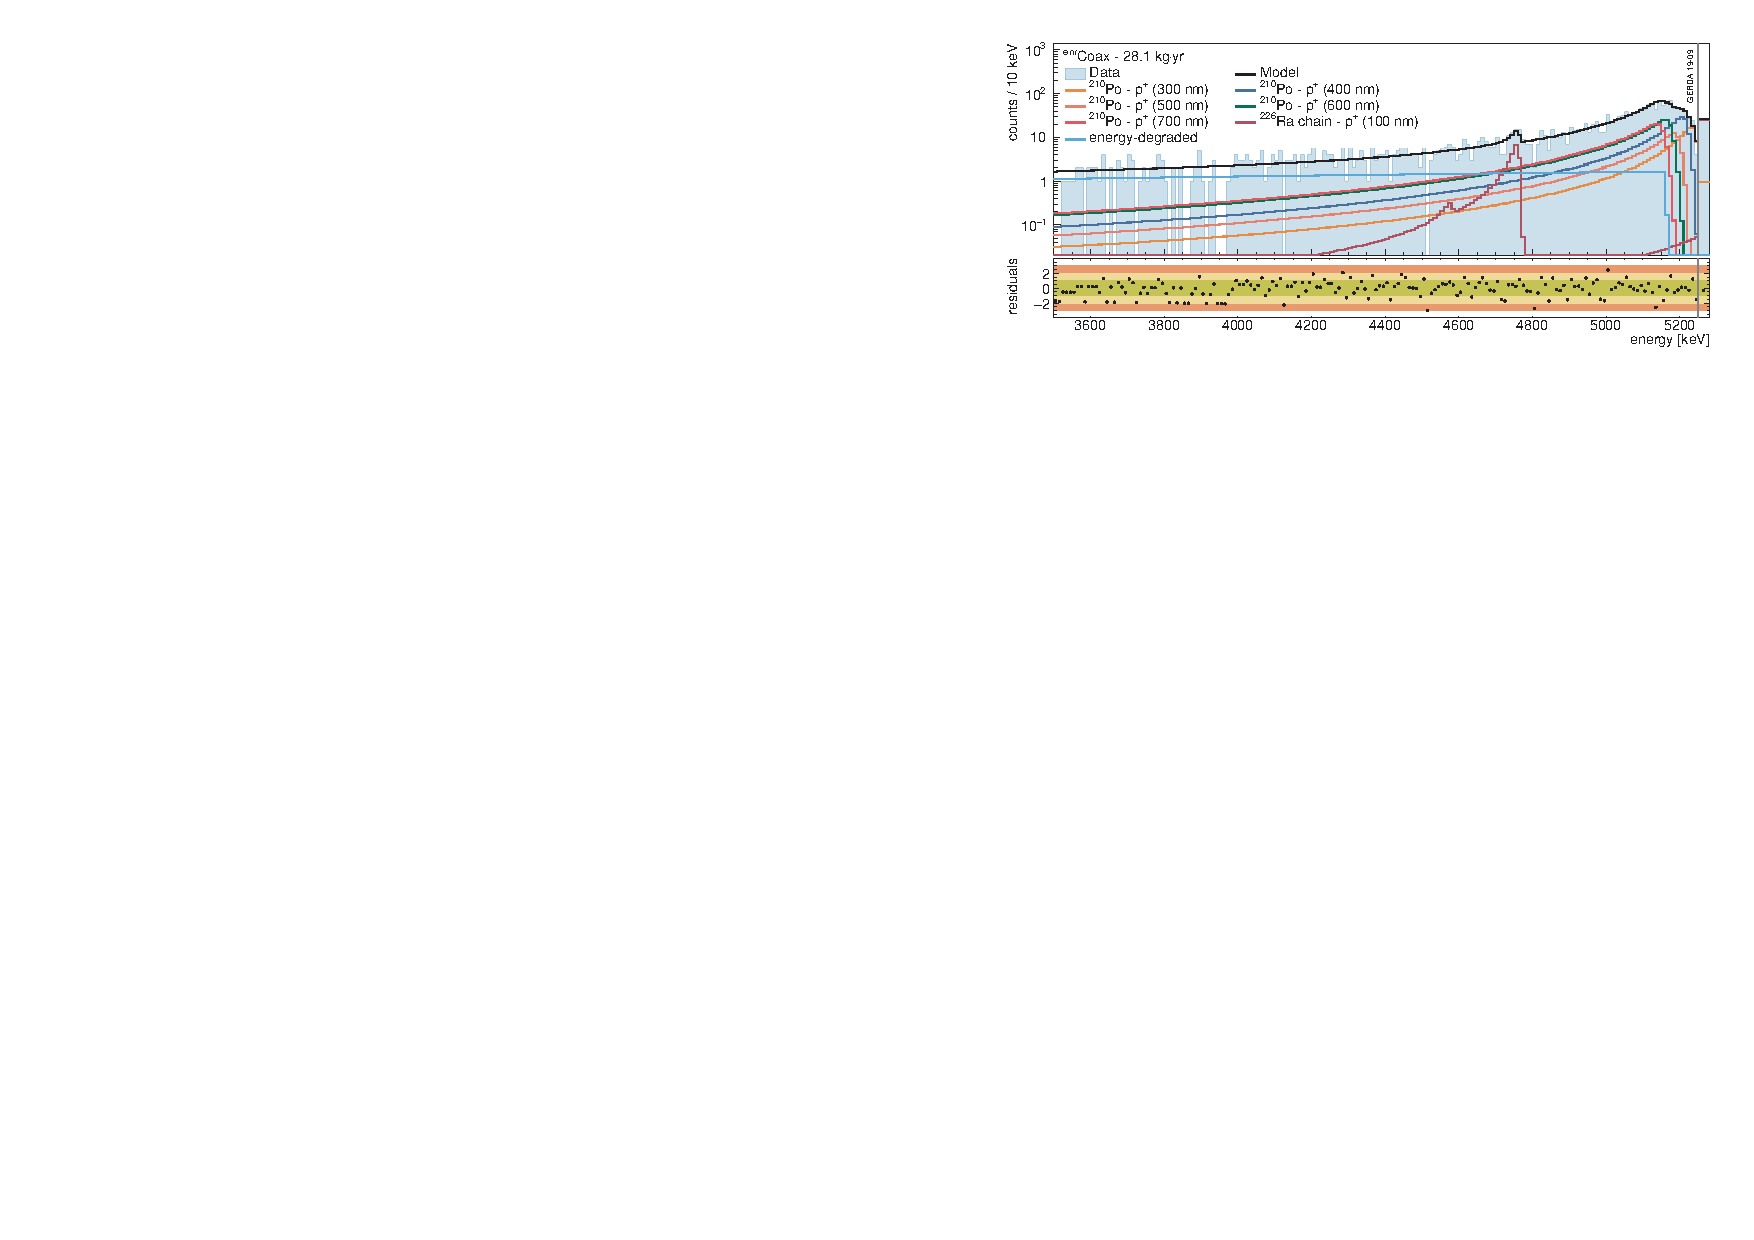
\includegraphics{plots/bkg/raw/ph2/results/amodel/amodel-enrCoax.pdf}
  \caption{%
    Fit results of the \a\ events background analysis for \enrBEGeII\
    (top) and \enrCoaxII\ (bottom). The last bin contains all events above
    5250~keV.
  }\label{fig:bkg:raw:ph2:amodel:resultsplot}
\end{figure}

\begin{table}
\centering
  \caption{%
    Fit results of the \a\ events background analysis for the
    \enrBEGeII\ and \enrCoaxII\ data sets. Values are given in counts in the
    full pdf range from 40~keV to 8000~keV.
  }\label{tab:bkg:raw:ph2:amodel:results}
  \begin{tabular}{rlccr@{ }l}
  \toprule
  \mr{2}{data set}   & \mr{2}{component} & contact & global mode & \mc{2}{marg.~mode}      \\
                     &                   & [nm]    & [cts]       & \mc{2}{68\% C.I.~[cts]} \\
  \midrule
  \mr{6}{\enrBEGeII} & \mr{4}{\Po}       & 400     & 49          & 50   & $[34,76]$        \\
                     &                   & 500     & 162         & 165  & $[107,222]$      \\
                     &                   & 600     & 346         & 342  & $[278,391]$      \\
                     &                   & comb.   & --          & 555  & $[523,586]$      \\
                     & \Ra\ chain        & 500     & 20          & 20   & $[15,29]$        \\
                     & energy-degraded   & --      & --          & 845  & $[698,948]$      \\
  \midrule
  \mr{8}{\enrCoaxII} & \mr{6}{\Po}       & 300     & 167         & 165  & $[140,208]$      \\
                     &                   & 400     & 363         & 368  & $[272,430]$      \\
                     &                   & 500     & 182         & 175  & $[83,338]$       \\
                     &                   & 600     & 433         & 420  & $[233,582]$      \\
                     &                   & 700     & 404         & 410  & $[295,537]$      \\
                     &                   & comb.   & --          & 1555 & $[1511,1609]$    \\
                     & \Ra\ chain        & 100     & 58          & 59   & $[49,70]$        \\
                     & energy-degraded   & --      & --          & 485  & $[426,599]$      \\
  \bottomrule
\end{tabular}

% vim: nowrap

\end{table}

\fillme{mention to time alpha}

% vim: tw=90
